\documentclass[a4paper,12pt]{article} % тип документа

%  Русский язык
\usepackage{multirow}
\usepackage{wrapfig}
\usepackage[T2A]{fontenc}			% кодировка
\usepackage[utf8]{inputenc}			% кодировка исходного текста
\usepackage[english,russian]{babel}	% локализация и переносы

\usepackage{indentfirst} %Красная строка
\usepackage[a4paper,top=1.3cm,bottom=2cm,left=1.5cm,right=1.5cm,marginparwidth=0.75cm]{geometry}
\usepackage[usenames]{color}
\usepackage{colortbl}
\usepackage{float}

\usepackage{graphicx}%картинки
\usepackage{wrapfig}%обтекание текстом теблиц и картинок
%гиперссылки
\usepackage{xcolor}
\usepackage{hyperref}
% Цвета для гиперссылок
\definecolor{linkcolor}{HTML}{799B03} % цвет ссылок
\definecolor{urlcolor}{HTML}{799B03} % цвет гиперссылок
\hypersetup{pdfstartview=FitH,
  linkcolor=linkcolor,
  urlcolor=urlcolor,
   colorlinks=true}
% Заметки
\usepackage{todonotes}

% Математика
\usepackage{amsmath,amsfonts,amssymb,amsthm,mathtools} 
\usepackage{hyperref}

\begin{document}

\begin{titlepage}
\begin{center}
    {\large МОСКОВСКИЙ ФИЗИКО-ТЕХНИЧЕСКИЙ ИНСТИТУТ (НАЦИОНАЛЬНЫЙ ИССЛЕДОВАТЕЛЬСКИЙ УНИВЕРСИТЕТ)}
\end{center}
\begin{center}
    {\largeФизтех-школа физики и исследований им. Ландау}
\end{center}

\vspace{3.5cm}

\begin{center}
    
\includegraphics[width=0.4\linewidth]{pictures/hv_full.png}
\end{center}
\vspace{0.1cm}
{\huge
\begin{center}
    {\bf Лабораторная работа 1.3.1}\\
    {Определение модуля Юнга на основе исследования деформаций растяжения и изгиба}
\end{center}
}
\vspace{2cm}
\begin{flushright}
{\LARGE Авторы:\\ Петров Олег \\
\vspace{0.2cm}
Б02-202}
\end{flushright}
\vspace{3.5cm}
\begin{center}
    Долгопрудный 2022
\end{center}
\end{titlepage}

\section{Aннотация}
\textbf{Цель работы:}Экспериментально получить зависимость между напряжением и деформацией
 для двух простейших напряженных состояний упругих тел: одностороннего сжатия и чистого изгиба;
 по результатам эксперимента вычислить модул Юнга.\\
\ \textbf{Оборудование:}в первой части - прибор Лермантова, проволка из исследуемого материала, зрительная трубка со шкалой,
набор грузов, микрометр,рулетка;  во второй части - стойка для изгибания балки, индикатор для измерения величин прогиба,
набор исследуемых стержней, грузы, линйка, штангенциркуль.
\section{Определение модуля Юнга по измерения растяжения проволки}
\subsection{Теоретические сведения}
Растяжение проволки соответствует напряженому состоянию вдоль одной оси, которое описывается формулой:
\begin{equation}
    \sigma = E \varepsilon, \ \ 
    \frac{F}{S} = E \frac{\Delta l}{l}
    \label{lermantov}
\end{equation}
Измерения производятся на установке Лермантова.
Направим зрительную трубку на зеркальце\dots.
Тогда учитывая параксиальность углов,
для расчета растяжения проволки справедлива формула:
\begin{equation}
    l = n\frac{r}{2h},
    \label{dlina}
\end{equation}
где h - расстояние от шкалы до зеркальца,
r - длина рычага, n - показания шкалы\\

\subsection{Эксперимантельная установка}

\begin{figure}[!h]
    \centering
    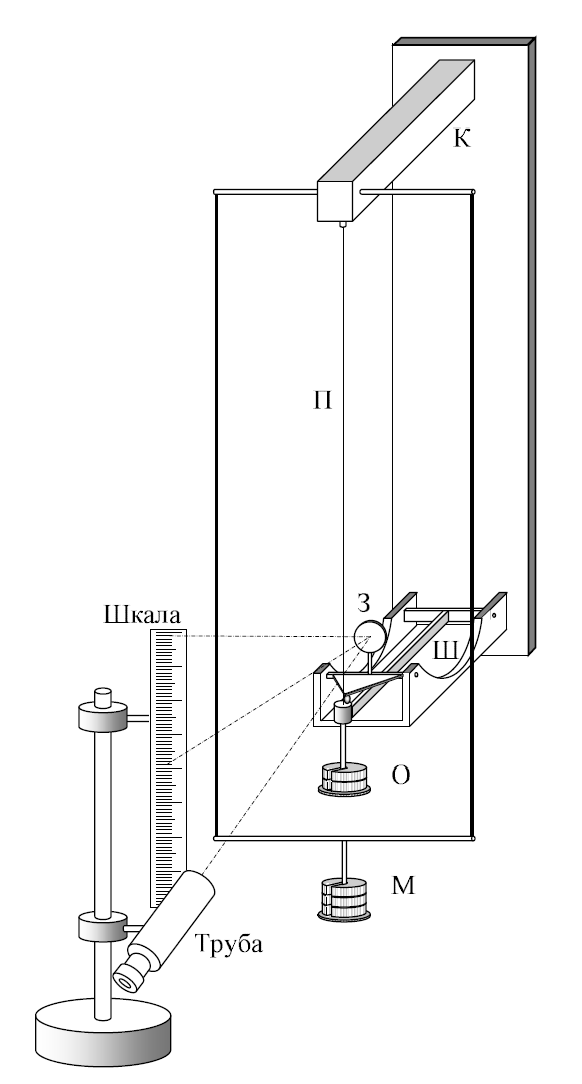
\includegraphics[height=0.35\textheight]{pictures/lermantov.png}
    \caption{Установка Лермантова и установка}
\end{figure}

Для определения модуля Юнга используется прибор Лермонтова,
схема которого изображена на рис. 1. Верхний конец проволоки П, из-
готовленной из исследуемого материала, прикреплен к консоли К, а
нижний - к цилиндру, которым оканчивается шарнирный кронштейн
Ш. На этот же цилиндр опирается рычаг r, связанный с зеркальцем
3. Таким образом, удлинение проволоки можно измерить по углу по-
ворота зеркальца.\\
Натяжение проволоки можно менять, перекладывая грузы с пло-
щадки М на площадку О и наоборот. Такая система позволяет исклю-
чить влияние деформации кронштейна К на точность измерений, так
как нагрузка на нем все время остается постоянной.

\subsection{Результаты эксперимента и обработка данных}

\begin{itemize}
    \item Сначалаа измерим параметры системы:
$$g=9.815 \pm 0.005 \ \text{м} \text{с}^2,\ \ \  h=138 \pm 1\ \text{мм},
\ \ \ r = 13 \pm 0.5 \ \text{мм},\ \ \  d_{\text{проволки}}=0.73 \pm 0.005\ \text{мм}$$
%\item Измеряем длину диаметра микрометрам в нескольких местах проволки во
%взаимной перпендикулярных напрялениях. Результаты заносим в табличку:\\
%%Таблица
%    \item Усредння по всем измерения получаем значение $d=$ мм.\\
%Погрешность оцениваем как:
%$$\sigma^d_\text{случ}=\sqrt{\sum_{i} (d_{i}-\langle d \rangle)^2 /N(N-1)}= \ \text{мм}, \ \ \sigma^d_\text{сист}=\Delta d= \ \text{мм}$$
%$$\sigma_{d}=\sqrt{\sigma^2_\text{случ}+\sigma^2_\text{сист}=\text{мм}, $$
 \item По полученным значениям вычисляем площадь и ее погрешность:
$$S=\frac{\pi d^2}{4}= 41.9 10^2 \ \text{мм}^2, \ \ \ \sigma_{S}=S\frac{2 \sigma_{d}}{d} = 0.6 \ 10^2 \ \text{мм}^2, 
\ \ \ \varepsilon _{S}=1.4 \%$$
 \item Измеряем длину проволки $l= 177\pm 1 $ см.\\
 \item Позаботимся о том, чтобы в процессе эксперимента не выйти за пределы области,
где удлинение проволки пропорционально ее натяжению. С учетом разрушительного напряжения:
$\sigma_{\text{разрушения}}= 900 \ H \cdot \text{мм}^{-2}$. Рассчитаем предельную массу груза,
 которую можно подвесить, чтобы не выйти из диапозона рабочих напряжений:\\ $m_{\text{предельная}}
 =0.3\cdot \sigma_{\text{разрушения}}S/g= 11.3 $ кг.

 \item С учетом полученного выше значения снимаем зависимость удлинения проволки от массы грузов 
грузов m при увеличении и уменьшении нагрузки. Данные заносим в таблицу ниже.
Расчет $\Delta l$ производим по формуле, а погрешность измерения $\Delta l$ оцениваем по формуле:
$$\varepsilon _{\Delta l} = \sqrt{\left( \dfrac{\sigma_{n}}{n}\right)^2 +
  \left(\dfrac{\sigma_r}{r}\right)^2+\left(\dfrac{\sigma_h}{h}\right)^2} \approx  \varepsilon_{r} = 3.8\%, \ \ \ 
\ \ \ \varepsilon_{\Delta m}=0.2\%$$
\begin{table}[!h]
    \begin{center}
    \label{table1}
    \begin{tabular}{|l|r|r|r|r|r|}\hline
        №  & $\Delta m \Downarrow $, гр & $m$, гр & $P$, Н & $n$, мм& $\Delta l$,мм\\ \hline
         1 &  245.8 &  2444.4 &  23.99 &  22.2 &  1.046\\ \hline 
         2 &  245.5 &  2198.6 &  21.58 &  21.1 &  0.994\\ \hline
         3 &  246.1 &  1953.1 &  19.17 &  20   &  0.942\\ \hline
         4 &  245.7 &  1707   &  16.76 &  18.9 &  0.890\\ \hline
         5 &  245.7 &  1461.3 &  14.34 &  17.6 &  0.829\\ \hline
         6 &  245.6 &  1215.6 &  11.93 &  16.5 &  0.777\\ \hline
         7 &  246.1 &  970    &  9.52  &  15.2 &  0.716\\ \hline
         8 &  245.2 &  723.9  &  7.11  &  14.2 &  0.669\\ \hline
         9 &  478.7 &  478.7  &  4.70  &  12.6 &  0.593\\ \hline
        \end{tabular}
    \caption{Измерения величин припонижении нагрузки}
    \end{center}
\end{table}


\begin{table}[!h]
    \begin{center}
    \begin{tabular}{|l|r|r|r|r|r|} \hline
           №  & $\Delta m \Uparrow $, гр & $m$, гр & $P$, Н & $n$, мм & $\Delta l$,mm \\ \hline
         1 &  246.1 &  970 &  9.52 &  15   &  0.707\\ \hline
         2 &  245.6 &  1215.6 &  11.93 &  16.3 &  0.768\\ \hline
         3 &  245.7 &  1461.3   &  14.34 &  17.6 &  0.829\\ \hline
         4 &  491.8 &  1953.1 &  19.17 &  19.9 &  0.937\\ \hline
         5 &  245.5 &  2198.6 &  21.58 &  21.1 &  0.994\\ \hline
         6 &  245.8 &  2444.4 &  23.99 &  22.2 &  1.046\\ \hline
        \end{tabular}
    \caption{Измерения величин при повышении нагрузки}
    \label{table1}
    \end{center}
\end{table}

 \item По полученным данным строим график зависимости $P(\Delta l)$ методом наименьших квадратов(МНК). Также
учтем что в недеформированном состоянии проволка, как правило, изогнута, и при малых нагрузках ее удлинение
определяется не растяжением, а выпрямлением.Поэтому исключим начальный участок зависимости из обработки данных.

\begin{figure}[!ht]
    \begin{center}
        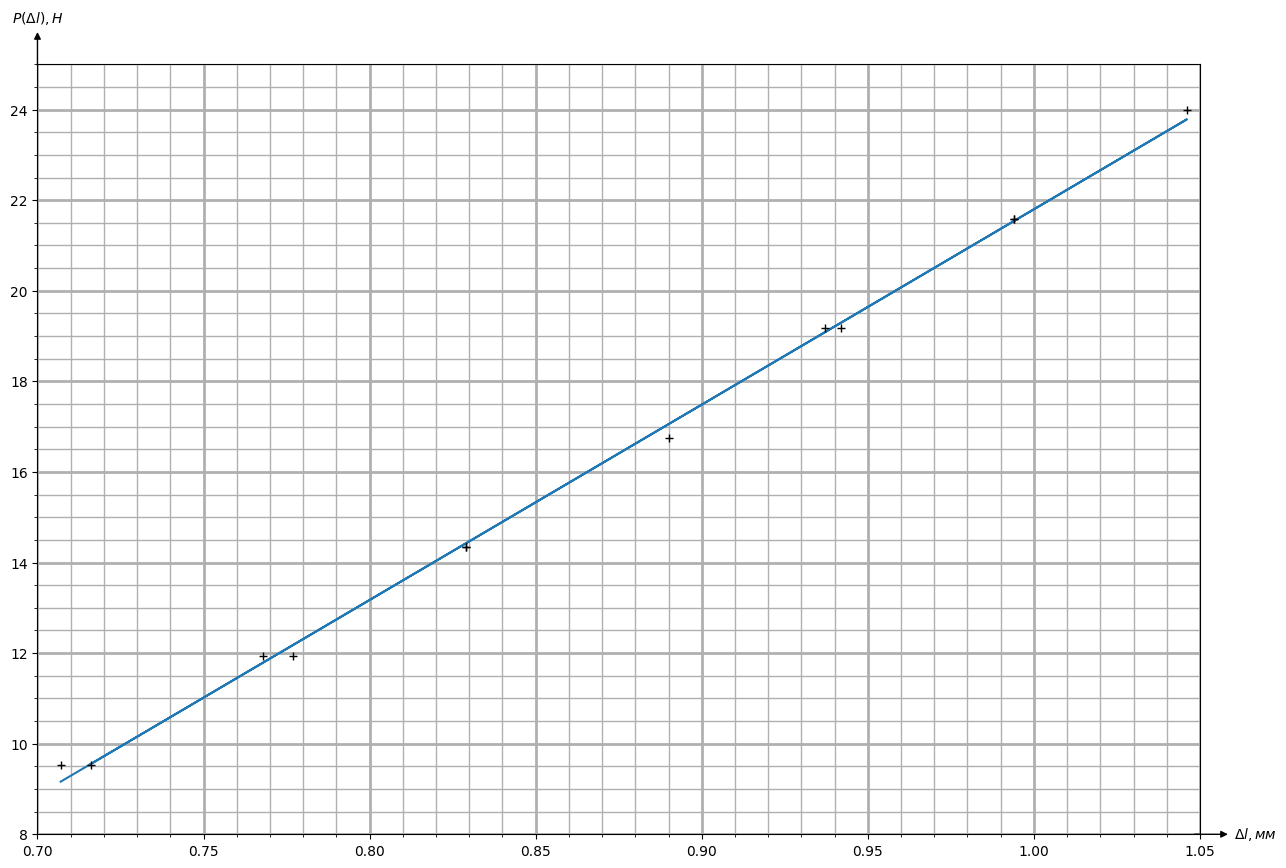
\includegraphics[width=1\textwidth]{pictures/graphic1.png}
        \caption{График зависимости $P(\Delta l)$ от $\Delta l$}
        \label{graphic1}
    \end{center}
\end{figure}

По формулам МНК находим коэффицент наклона графика для прямой и его случайную погрешность.
Для коэффицента наклона графика имеем:
$$k=\dfrac{\langle P \Delta l \rangle-\langle P \rangle \langle \Delta l \rangle}
{\langle \Delta l^2 \rangle - \langle \Delta l \rangle^2}
=43.1 \ H \cdot \text{мм}$$
Для систематической и случайной относительной погрешности имеем:
$$\varepsilon_k^\text{случ}=\frac{1}{k\sqrt{N-2}}\sqrt{\frac{\langle P^2 \rangle - \langle P \rangle^2}
{\langle \Delta l^2 \rangle - \langle \Delta l \rangle^2} - k^2 }=4.3 \%, \ \ \ \ 
\varepsilon_k^\text{сист}=\sqrt{\varepsilon^2_{P}+\varepsilon^2_{\Delta l}}\approx \varepsilon_{\Delta l} = 3.8 \% $$
$$\varepsilon_k=\sqrt{\varepsilon_\text{сист}^2+\varepsilon_\text{случ}^2}=5.7\% $$
    \item С учетом формул выше получаем, как выражается модуль Юнга через коэффицент наклона графика,
и выражение для его погрешности:
$$ E = \frac{k l}{S} = 180 \ \text{ГПа}$$
$$\varepsilon_{E}=\sqrt{\varepsilon^2_{S}+\varepsilon^2_{k}+\varepsilon^2_{l}} \approx \varepsilon_{k} = 5.8 \%, \ \ \ \sigma_{E}= \varepsilon \cdot E = 1 \ \text{ГПа}$$
По итогу получаем значение для модуля Юнга проволки: $E = 180 \pm 10$ ГПа и относительной погрешность $\varepsilon_{E}= 6\%$
\end{itemize}

\section{Определение модуля Юнга по измерению изгиба балки}

\subsection{Теоретические сведения}
Модуль Юнга материала стержня $E$ связан со стрелой прогиба $y_{max}$ как:
\begin{equation}\label{balka}
    E=\frac{Pl^3}{4ab^3y_{max}}
\end{equation}
где $P$ - нагрузка на стержень, $l$ - расстояние меду точками опоры,
$a$ - ширина балки ,$b$ - высота балки

\subsection{Экспериментальная установка}

\begin{figure}[!ht]
    \centering
    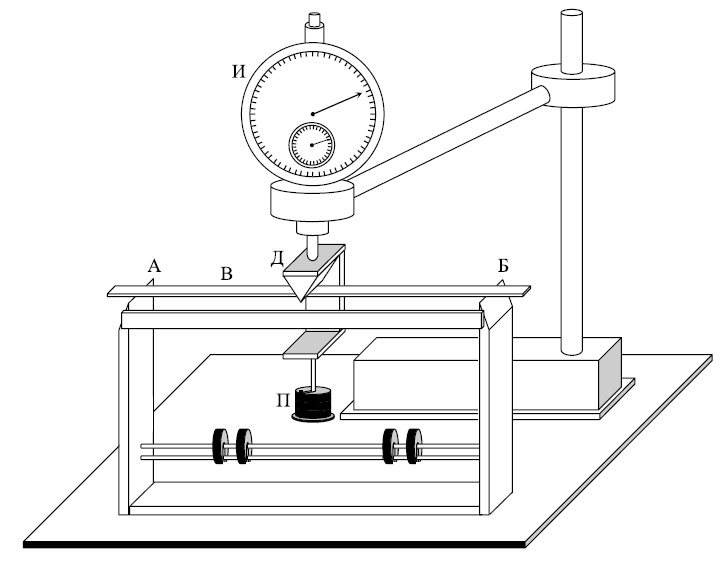
\includegraphics[scale=1]{pictures/balka.png}
    \caption{Установка Лермантова и установка}
\end{figure}

Экспериментальная установка состоит из прочной стойки с опорным-
ми призмами А и Б (рис. 2). На ребра призм опирается исследуемый
стержень (балка) В. В середине стержня на призме Д подвешена пло-
щадка П с грузами. Измерять стрелу прогиба можно с помощью инди-
катара И, укрепляемого на отдельной штанге. Полный оборот большой
стрелки индикатора соответствует 1 мм и одному делению малого циферблата.

\subsection{Результаты эксперимента и обработка данных}

\begin{itemize}
    \item Измерим расстояние между опорами $l= 51 \pm 0.5 $мм, $\varepsilon_{l}= 1 \%$
    \item Измерим высоту $d$ и ширину $a$ балок из различных материалов и занесем данные в таблицу.

\begin{table}[!h]
    \begin{center}  
    \begin{tabular}{|l|l|l|l|l|l|l|l|l|l|l|} \hline
        $N1$,латунь & 1    & 2     & 3    & 4    & 5    & 6    & 7    & 8    & 9    & 10   \\ \hline
        $a$, см     & 2.16 & 2.14  & 2.14 & 2.14 & 2.14 & 2.14 & 2.15 & 2.14 & 2.14 & 2.14 \\ \hline
        $b$, см     & 0.38 & 0.39  & 0.39 & 0.39 & 0.39 & 0;38 & 0.39 & 0.39 & 0.39 & 0.39 \\ \hline
        $N2$,сталь  & 1    & 2     & 3    & 4    & 5    & 6    & 7    & 8    & 9    & 10   \\ \hline
        $a$, см     & 2.09 & 2.1   & 2.12 & 2.12 & 2.12 & 2.14 & 2.11 & 2.11 & 2.12 & 2.11 \\ \hline
        $b$, см     & 0.37 & 0.375 & 0.37 & 0.37 & 0.37 & 0.37 & 0.37 & 0.37 & 0.37 & 0.37 \\ \hline
    \end{tabular}
    \end{center}
\end{table}

За истинное значение примим среднее по всей выборке. Погрешности измерений оцениваем по формулам:
    $$\sigma^a_\text{случ}=\sqrt{\sum_{i} (a_{i}-\langle a \rangle)^2 /N(N-1)}, \ \ \sigma^a_\text{сист}=\Delta a$$
$$\sigma_{a}=\sqrt{\sigma^2_\text{случ}+\sigma^2_\text{сист}}$$
Получаем значения для латуни: $a_{\text{лат}} = 2.143 \pm 0.005 \ \text{см},\  b_{\text{лат}}=0.390 \pm 0.005 \ \text{см}$
и для относительных погрешностей имеем: $\varepsilon_{a_{\text{лат}}}=0.2 \%, \  \varepsilon_{b_{\text{лат}}} = 1.2 \% $\\
Получаем значения для латуни: $a_{\text{сталь}} = 2.118 \pm 0.005 \ \text{см},\  b_{\text{сталь}}=0.370 \pm 0.005 \ \text{см}$
и для относительных погрешностей имеем: $\varepsilon_{a_{\text{сталь}}}=0.2 \%, \  \varepsilon_{b_{\text{сталь}}} = 1.3 \% $\\
Тогда для моментов инерции поперечного сечения балки относительно оси, проходящей через
среднюю линию балки имеем:
$$I=\frac{ab^3}{12},\ \ \ \varepsilon_{I}=\sqrt{\varepsilon^2_{a}+9\varepsilon_{b}^2}\approx 3 \varepsilon_{b}$$\\
Значение для латуни: $I_{\text{лат}} = 10.5 \pm 0.4\ 10^{-3} \ \text{см}^4, \varepsilon_{I_{\text{лат}}}=3.6 \% $\\
Значение для стали: $I_{\text{сталь}} = 8.9 \pm 0.3 \ 10^{-3} \ \text{см}^4, \varepsilon_{I_{\text{сталь}}}=4.0 \% $\\
    \item Кладем исследуемую балку на стойку. Устанавливаем индикатор в центре балки
 и снимаем зависимость стрелы прогиба $\Delta y_{max}$ от величины нагрузки$P$. Проделываем эти измерения
 при возрастающей и убывающей нагрузки, заносим данные в таблицу. Заносим эти данные в таблицу
 и строим по этим точкам график методом намименьших квадратов (МНК).

 \begin{table}[!h]
    \begin{center}
    \begin{tabular}{|l|l|l|l|l|l|l|l|}\hline
    $m$, гр & $\Delta_{y_{\text{max}}} \Uparrow $,cм & $P$, Н   & $y_{max}$, cм & $m$, гр & $\Delta_{y_{\text{max}}} \Downarrow $,cм & $P$, Н   & $y_{max}$, cм \\ \hline
    482.5 & 1.15  & 4.736  & 1.15  & 478.2  & -1.17   & 28.885 & 7.21 \\ \hline
    503.1 & 1.23  & 9.674  & 2.38  & 511    & -1.24   & 24.191 & 6.04 \\ \hline
    501.3 & 1.28  & 14.595 & 3.66  & 466.7  & -1.13   & 19.176 & 4.8  \\ \hline
    466.7 & 1.14  & 19.176 & 4.8   & 501.3  & -1.23   & 14.595 & 3.67 \\ \hline
    511   & 1.25  & 24.191 & 6.05  & 503.1  & -1.23   & 9.674  & 2.44 \\ \hline
    478.2 & 1.16  & 28.885 & 7.21  & 482.5  & 1.14    & 4.736  & 1.21 \\ \hline
    \end{tabular}
    \caption{Величина прогиба в зависимости от массы при повышении $\Uparrow $ и при понижении массы $\Downarrow $ для латунной балки}
    \end{center}
\end{table}

    \item Исследуем, насколько существенна зависимость результата от положения точки 
приложения изгибающей силы $P$. Сместим т. давления на 2-3 см от середины балки 
проведем аналогичные измерения. Построим по этим точкам прямую на том же графике пользуясь (МНК).

\begin{table}[!h]
    \begin{center}
    \begin{tabular}{|l|l|l|l|} \hline
    $m$,гр & $\Delta_{y_{\text{max}}}$,cм & $P$, Н   & $y_{max}$, cм \\ \hline
    482.5 & 1.15 & 4.736  & 1.15 \\ \hline
    503.1 & 1.22 & 9.674  & 2.37 \\ \hline 
    501.3 & 1.25 & 14.595 & 3.62 \\ \hline
    466.7 & 1.13 & 19.176 & 4.75 \\ \hline
    511   & 1.23 & 24.191 & 5.98 \\ \hline
    478.2 & 1.12 & 28.885 & 7.1 \\ \hline
    \end{tabular}
    \caption{Величина прогиба в зависимости от массы при при смещении т. пприложения сил на 2-3 см}
    \end{center}
\end{table}

\begin{figure}[!h]
    \begin{center}
        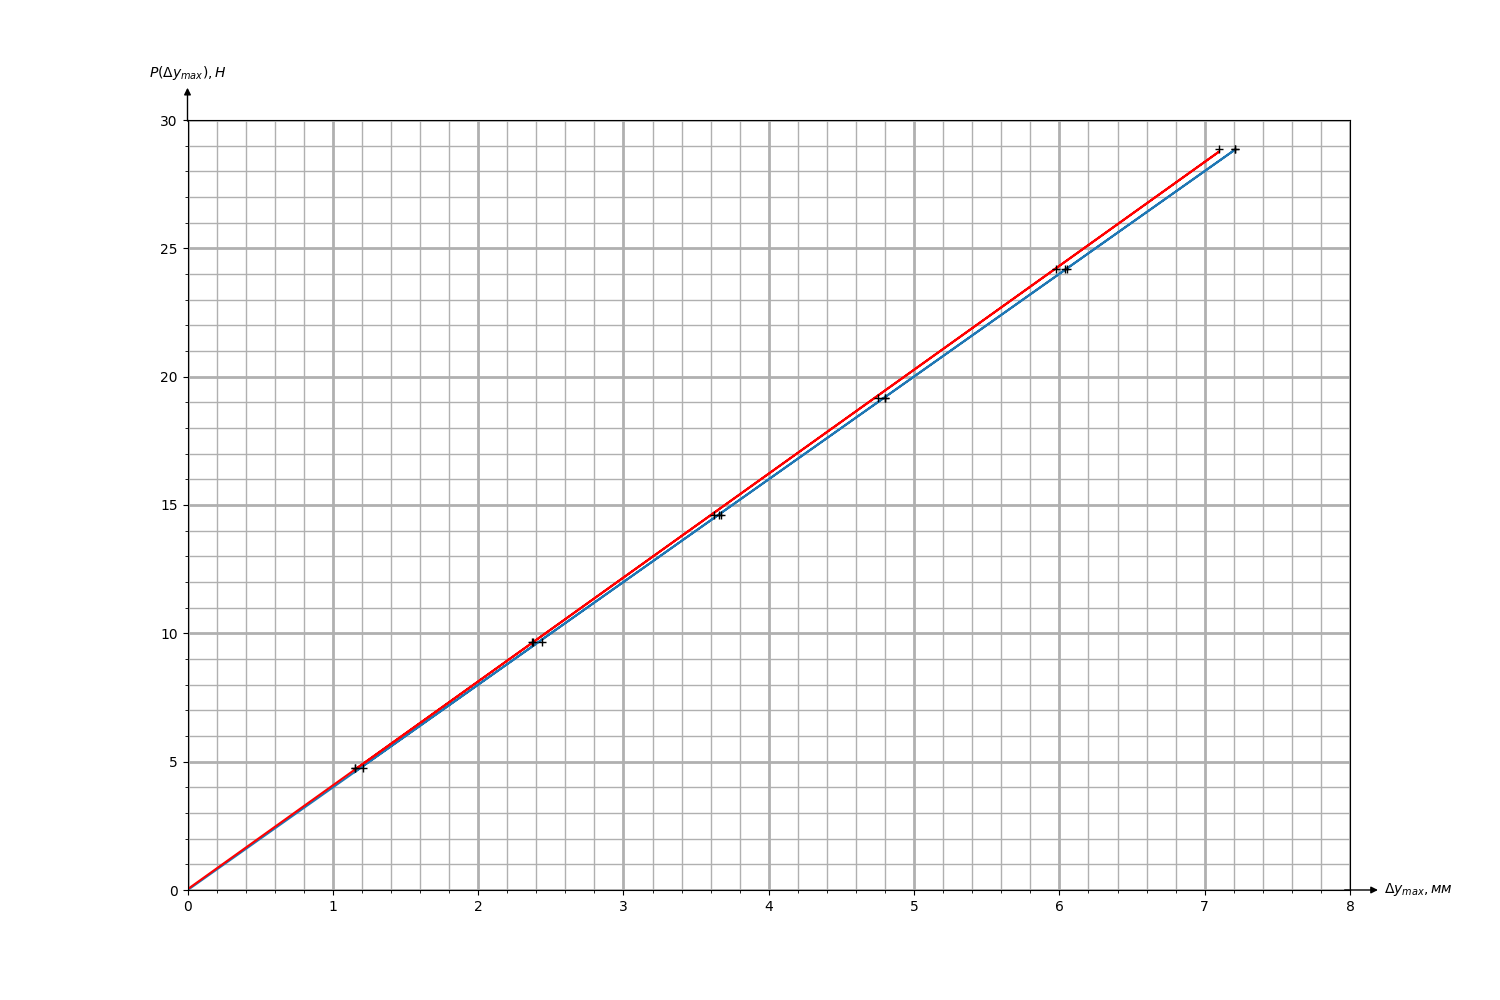
\includegraphics[width=1\textwidth]{pictures/graphic12b.png}
        \caption{График зависимости $P(y_{max})$ от $y_{max}$ для латунной балки при прямом и обратном ходе и при смещении т. давления}
        \label{graphic1yyyb}
    \end{center}
\end{figure}

Как видно точки первого и второго графика лежат практически на одной прямой, коэффиценты наклона находим по формулам:
$$k=\dfrac{\langle P \Delta y_{max} \rangle-\langle P \rangle \langle \Delta y_{max} \rangle}
{\langle y^2_{max} \rangle - \langle  y_{max} \rangle^2}$$\\
Учтем, что $\varepsilon_{\Delta_{y_{\text{max}}}} \approx 1.6 \%$, а $\varepsilon_{m} \approx 0.01 \%$\\
Итоговую погрешность измерения $\varepsilon_{y_{\text{max}}}$ посчитаем как усредненную по всем значениям $N$
$\varepsilon_{y_{\text{max}}}v= \langle \sqrt{N}\varepsilon_{\Delta_{y_{\text{max}}}} \rangle = 3.6 \% $\\
Для оценики систематической и случайной относительной погрешности пользуемся формулами получаем:
$$\varepsilon_k^\text{случ}=\frac{1}{k\sqrt{N-2}}\sqrt{\frac{\langle P^2 \rangle - \langle P \rangle^2}
{\langle y^2_{max} \rangle - \langle  y_{max} \rangle^2} - k^2} = 0.3 \%, \ \ \ 
\varepsilon_k^\text{сист}=\sqrt{\varepsilon^2_{P}+\varepsilon^2_{y_{max}}} \approx \varepsilon_{y_{max}} = 3.6 \% $$
$$\varepsilon_k=\sqrt{\varepsilon_\text{сист}^2+\varepsilon_\text{случ}^2} \approx \varepsilon_{y_{max}}= 3.6 \% $$\\
Для итоговых значений коэффицентов наклона имеем:
$$k_{\text{латунь}}=4.00 \pm 0.14 \ \text{H}/\text{см}, \ \ \
k_{\text{латунь,сдвиг}}=4.04 \pm 0.14 \ \text{H}/\text{см} $$
Как видно, коэффиценты наклона при смещении на 2-3 см и в середине практически совпадают и 
находятся в пределах погрешности друг друга.
    \item Теперь посчитаем модуль Юнга по формуле $\href{balka}{3}$:
$$E_{\text{латунь}} = \frac{k l^3}{48 I_{\text{латунь}}}=105 \ \text{ГПа}, \ \ \ 
\varepsilon_{E}=\sqrt{\varepsilon^2_{k}+9\varepsilon^2_{l}+\varepsilon^2_{I}=} = 5 \% $$
По итогу получаем значение: $E_{\text{латунь}}= 105 \pm 5$ Гпа.
    \item Аналогичные измерения зависимости нагрузки от стелы прогиба проводим для балки из стали.
Данные заносим в таблицу:

\begin{table}[!h]
    \begin{center}
    \begin{tabular}{|l|l|l|l|} \hline
    $m$,гр & $\Delta y_{\text{max}}$,cм & $P$, Н   & $y_{max}$, cм \\ \hline
    482.5   & 0.65 & 4.736   & 0.65   \\ \hline 
    503.1   & 0.7  & 9.674   & 1.35   \\ \hline
    501.3   & 0.67 & 14.595  & 2.02   \\ \hline
    466.7   & 0.63 & 19.176  & 2.65   \\ \hline
    511     & 0.7  & 24.191  & 3.35   \\ \hline
    478.2   & 0.65 & 28.885  & 4      \\ \hline
    \end{tabular}
    \caption{Величина прогиба в зависимости от массы для стальной балки}
    \end{center}
\end{table}

\begin{figure}[h]
    \begin{center}
    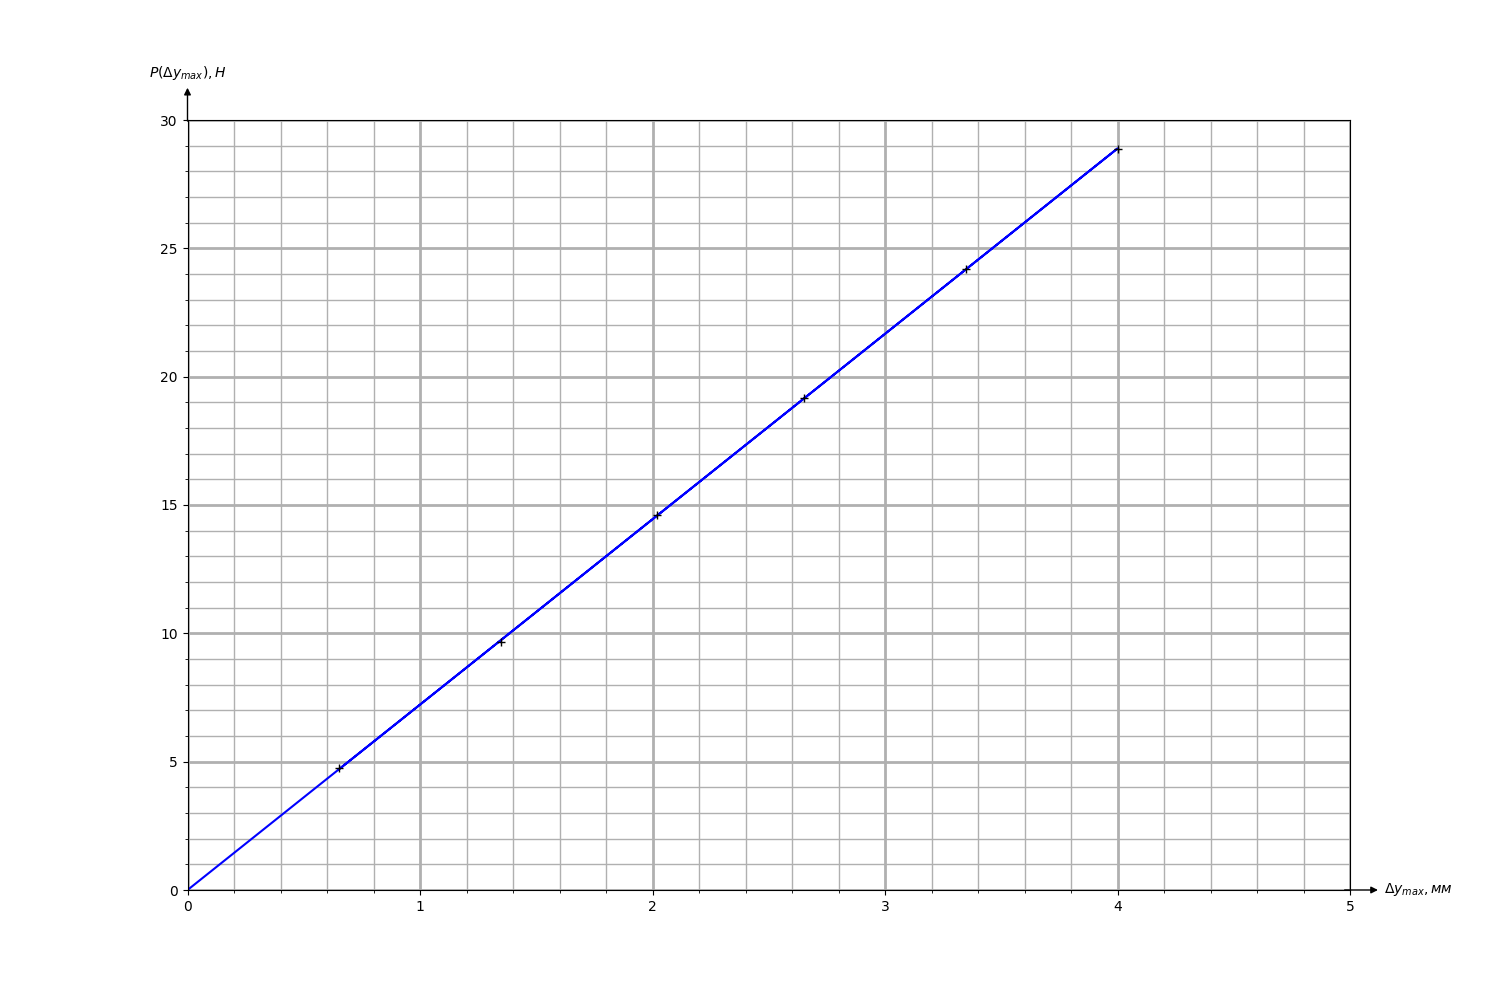
\includegraphics[width=1\textwidth]{pictures/graphic3b.png}
    \caption{График зависимости $P(y_{max})$ от $y_{max}$ для стальной балки}
    \end{center}
\end{figure}

По полученным данным строим график методом наименьших квадратов(МНК).\\
Пользуясь формулами для МНК аналогично случаю латунной балки находим значение коэффицента наклона и его погрешность:
$$k = 7.2 \pm 0.4 \ \text{H}/\text{см}, \ \ \ \varepsilon_{k}=6 \% $$
Теперь мы можем рассчитать модуль Юнга для стальной балки и его погрешность:
$$E_{\text{сталь}} = \frac{k l^3}{48 I_{\text{сталь}}}=224 \ \text{ГПа}, \ \ \ 
\varepsilon_{E}=\sqrt{\varepsilon^2_{k}+9\varepsilon^2_{l}+\varepsilon^2_{I}} = 7\%$$
По итогу получаем значение $E_{\text{сталь}}= 224 \pm 15$ Гпа.

\end{itemize}

\section{Выводы}

В результате выполнения работы было поддтверждено несколько теоретических зависимостей. Получены ожидаемые
линейные зависимости между стрелой прогиба и весом нагрузки.\\
\ В первой части работы были получено значение модуля Юнга проволки:
$E = 180 \pm 10$ Гпа которое в пределах погрешности  $\varepsilon_{E}= 6 \%$ совпадает с табличным значением для стали и железа.\\
\ Во второй части работы получены значения для модулей Юнга стали $E_{\text{сталь}}= 224 \pm 15$ Гпа и латуни $E_{\text{латунь}}= 105 \pm 5$ Гпа соответственно, 
которые совпадают с табличными значениями в пределах погрешности.

\end{document}